\documentclass{beamer}

\usepackage{amsmath,amssymb}
\usepackage{stmaryrd}
\usepackage{proof}
\usepackage{graphicx}
\usepackage{tikz}
\usetikzlibrary{trees}

%% ODER: format ==         = "\mathrel{==}"
%% ODER: format /=         = "\neq "
%
%
\makeatletter
\@ifundefined{lhs2tex.lhs2tex.sty.read}%
  {\@namedef{lhs2tex.lhs2tex.sty.read}{}%
   \newcommand\SkipToFmtEnd{}%
   \newcommand\EndFmtInput{}%
   \long\def\SkipToFmtEnd#1\EndFmtInput{}%
  }\SkipToFmtEnd

\newcommand\ReadOnlyOnce[1]{\@ifundefined{#1}{\@namedef{#1}{}}\SkipToFmtEnd}
\usepackage{amstext}
\usepackage{amssymb}
\usepackage{stmaryrd}
\DeclareFontFamily{OT1}{cmtex}{}
\DeclareFontShape{OT1}{cmtex}{m}{n}
  {<5><6><7><8>cmtex8
   <9>cmtex9
   <10><10.95><12><14.4><17.28><20.74><24.88>cmtex10}{}
\DeclareFontShape{OT1}{cmtex}{m}{it}
  {<-> ssub * cmtt/m/it}{}
\newcommand{\texfamily}{\fontfamily{cmtex}\selectfont}
\DeclareFontShape{OT1}{cmtt}{bx}{n}
  {<5><6><7><8>cmtt8
   <9>cmbtt9
   <10><10.95><12><14.4><17.28><20.74><24.88>cmbtt10}{}
\DeclareFontShape{OT1}{cmtex}{bx}{n}
  {<-> ssub * cmtt/bx/n}{}
\newcommand{\tex}[1]{\text{\texfamily#1}}	% NEU

\newcommand{\Sp}{\hskip.33334em\relax}


\newcommand{\Conid}[1]{\mathit{#1}}
\newcommand{\Varid}[1]{\mathit{#1}}
\newcommand{\anonymous}{\kern0.06em \vbox{\hrule\@width.5em}}
\newcommand{\plus}{\mathbin{+\!\!\!+}}
\newcommand{\bind}{\mathbin{>\!\!\!>\mkern-6.7mu=}}
\newcommand{\rbind}{\mathbin{=\mkern-6.7mu<\!\!\!<}}% suggested by Neil Mitchell
\newcommand{\sequ}{\mathbin{>\!\!\!>}}
\renewcommand{\leq}{\leqslant}
\renewcommand{\geq}{\geqslant}
\usepackage{polytable}

%mathindent has to be defined
\@ifundefined{mathindent}%
  {\newdimen\mathindent\mathindent\leftmargini}%
  {}%

\def\resethooks{%
  \global\let\SaveRestoreHook\empty
  \global\let\ColumnHook\empty}
\newcommand*{\savecolumns}[1][default]%
  {\g@addto@macro\SaveRestoreHook{\savecolumns[#1]}}
\newcommand*{\restorecolumns}[1][default]%
  {\g@addto@macro\SaveRestoreHook{\restorecolumns[#1]}}
\newcommand*{\aligncolumn}[2]%
  {\g@addto@macro\ColumnHook{\column{#1}{#2}}}

\resethooks

\newcommand{\onelinecommentchars}{\quad-{}- }
\newcommand{\commentbeginchars}{\enskip\{-}
\newcommand{\commentendchars}{-\}\enskip}

\newcommand{\visiblecomments}{%
  \let\onelinecomment=\onelinecommentchars
  \let\commentbegin=\commentbeginchars
  \let\commentend=\commentendchars}

\newcommand{\invisiblecomments}{%
  \let\onelinecomment=\empty
  \let\commentbegin=\empty
  \let\commentend=\empty}

\visiblecomments

\newlength{\blanklineskip}
\setlength{\blanklineskip}{0.66084ex}

\newcommand{\hsindent}[1]{\quad}% default is fixed indentation
\let\hspre\empty
\let\hspost\empty
\newcommand{\NB}{\textbf{NB}}
\newcommand{\Todo}[1]{$\langle$\textbf{To do:}~#1$\rangle$}

\EndFmtInput
\makeatother
%
%
%
%
%
%
% This package provides two environments suitable to take the place
% of hscode, called "plainhscode" and "arrayhscode". 
%
% The plain environment surrounds each code block by vertical space,
% and it uses \abovedisplayskip and \belowdisplayskip to get spacing
% similar to formulas. Note that if these dimensions are changed,
% the spacing around displayed math formulas changes as well.
% All code is indented using \leftskip.
%
% Changed 19.08.2004 to reflect changes in colorcode. Should work with
% CodeGroup.sty.
%
\ReadOnlyOnce{polycode.fmt}%
\makeatletter

\newcommand{\hsnewpar}[1]%
  {{\parskip=0pt\parindent=0pt\par\vskip #1\noindent}}

% can be used, for instance, to redefine the code size, by setting the
% command to \small or something alike
\newcommand{\hscodestyle}{}

% The command \sethscode can be used to switch the code formatting
% behaviour by mapping the hscode environment in the subst directive
% to a new LaTeX environment.

\newcommand{\sethscode}[1]%
  {\expandafter\let\expandafter\hscode\csname #1\endcsname
   \expandafter\let\expandafter\endhscode\csname end#1\endcsname}

% "compatibility" mode restores the non-polycode.fmt layout.

\newenvironment{compathscode}%
  {\par\noindent
   \advance\leftskip\mathindent
   \hscodestyle
   \let\\=\@normalcr
   \let\hspre\(\let\hspost\)%
   \pboxed}%
  {\endpboxed\)%
   \par\noindent
   \ignorespacesafterend}

\newcommand{\compaths}{\sethscode{compathscode}}

% "plain" mode is the proposed default.
% It should now work with \centering.
% This required some changes. The old version
% is still available for reference as oldplainhscode.

\newenvironment{plainhscode}%
  {\hsnewpar\abovedisplayskip
   \advance\leftskip\mathindent
   \hscodestyle
   \let\hspre\(\let\hspost\)%
   \pboxed}%
  {\endpboxed%
   \hsnewpar\belowdisplayskip
   \ignorespacesafterend}

\newenvironment{oldplainhscode}%
  {\hsnewpar\abovedisplayskip
   \advance\leftskip\mathindent
   \hscodestyle
   \let\\=\@normalcr
   \(\pboxed}%
  {\endpboxed\)%
   \hsnewpar\belowdisplayskip
   \ignorespacesafterend}

% Here, we make plainhscode the default environment.

\newcommand{\plainhs}{\sethscode{plainhscode}}
\newcommand{\oldplainhs}{\sethscode{oldplainhscode}}
\plainhs

% The arrayhscode is like plain, but makes use of polytable's
% parray environment which disallows page breaks in code blocks.

\newenvironment{arrayhscode}%
  {\hsnewpar\abovedisplayskip
   \advance\leftskip\mathindent
   \hscodestyle
   \let\\=\@normalcr
   \(\parray}%
  {\endparray\)%
   \hsnewpar\belowdisplayskip
   \ignorespacesafterend}

\newcommand{\arrayhs}{\sethscode{arrayhscode}}

% The mathhscode environment also makes use of polytable's parray 
% environment. It is supposed to be used only inside math mode 
% (I used it to typeset the type rules in my thesis).

\newenvironment{mathhscode}%
  {\parray}{\endparray}

\newcommand{\mathhs}{\sethscode{mathhscode}}

% texths is similar to mathhs, but works in text mode.

\newenvironment{texthscode}%
  {\(\parray}{\endparray\)}

\newcommand{\texths}{\sethscode{texthscode}}

% The framed environment places code in a framed box.

\def\codeframewidth{\arrayrulewidth}
\RequirePackage{calc}

\newenvironment{framedhscode}%
  {\parskip=\abovedisplayskip\par\noindent
   \hscodestyle
   \arrayrulewidth=\codeframewidth
   \tabular{@{}|p{\linewidth-2\arraycolsep-2\arrayrulewidth-2pt}|@{}}%
   \hline\framedhslinecorrect\\{-1.5ex}%
   \let\endoflinesave=\\
   \let\\=\@normalcr
   \(\pboxed}%
  {\endpboxed\)%
   \framedhslinecorrect\endoflinesave{.5ex}\hline
   \endtabular
   \parskip=\belowdisplayskip\par\noindent
   \ignorespacesafterend}

\newcommand{\framedhslinecorrect}[2]%
  {#1[#2]}

\newcommand{\framedhs}{\sethscode{framedhscode}}

% The inlinehscode environment is an experimental environment
% that can be used to typeset displayed code inline.

\newenvironment{inlinehscode}%
  {\(\def\column##1##2{}%
   \let\>\undefined\let\<\undefined\let\\\undefined
   \newcommand\>[1][]{}\newcommand\<[1][]{}\newcommand\\[1][]{}%
   \def\fromto##1##2##3{##3}%
   \def\nextline{}}{\) }%

\newcommand{\inlinehs}{\sethscode{inlinehscode}}

% The joincode environment is a separate environment that
% can be used to surround and thereby connect multiple code
% blocks.

\newenvironment{joincode}%
  {\let\orighscode=\hscode
   \let\origendhscode=\endhscode
   \def\endhscode{\def\hscode{\endgroup\def\@currenvir{hscode}\\}\begingroup}
   %\let\SaveRestoreHook=\empty
   %\let\ColumnHook=\empty
   %\let\resethooks=\empty
   \orighscode\def\hscode{\endgroup\def\@currenvir{hscode}}}%
  {\origendhscode
   \global\let\hscode=\orighscode
   \global\let\endhscode=\origendhscode}%

\makeatother
\EndFmtInput
%


\title{Certified Bit-Coded Regular Expression Parsing} 

\author{\textbf{Rodrigo Ribeiro}\inst{1} \and Andr\'e Rauber Du Bois\inst{2}} 
\institute 
{
\inst{1} Departament of Computer Science\\
         Universidade Federal de Ouro Preto \\ $\,$ \\
\inst{2} Departament of Computer Science\\
         Universidade Federal de Pelotas
}
\date{\today}



\DeclareMathAlphabet{\mathkw}{OT1}{cmss}{bx}{n}

\usepackage{color}
\newcommand{\redFG}[1]{\textcolor[rgb]{0.6,0,0}{#1}}
\newcommand{\greenFG}[1]{\textcolor[rgb]{0,0.4,0}{#1}}
\newcommand{\blueFG}[1]{\textcolor[rgb]{0,0,0.8}{#1}}
\newcommand{\orangeFG}[1]{\textcolor[rgb]{0.8,0.4,0}{#1}}
\newcommand{\purpleFG}[1]{\textcolor[rgb]{0.4,0,0.4}{#1}}
\newcommand{\yellowFG}[1]{\textcolor{yellow}{#1}}
\newcommand{\brownFG}[1]{\textcolor[rgb]{0.5,0.2,0.2}{#1}}
\newcommand{\blackFG}[1]{\textcolor[rgb]{0,0,0}{#1}}
\newcommand{\whiteFG}[1]{\textcolor[rgb]{1,1,1}{#1}}
\newcommand{\yellowBG}[1]{\colorbox[rgb]{1,1,0.2}{#1}}
\newcommand{\brownBG}[1]{\colorbox[rgb]{1.0,0.7,0.4}{#1}}

\newcommand{\ColourStuff}{
  \newcommand{\red}{\redFG}
  \newcommand{\green}{\greenFG}
  \newcommand{\blue}{\blueFG}
  \newcommand{\orange}{\orangeFG}
  \newcommand{\purple}{\purpleFG}
  \newcommand{\yellow}{\yellowFG}
  \newcommand{\brown}{\brownFG}
  \newcommand{\black}{\blackFG}
  \newcommand{\white}{\whiteFG}
}

\newcommand{\MonochromeStuff}{
  \newcommand{\red}{\blackFG}
  \newcommand{\green}{\blackFG}
  \newcommand{\blue}{\blackFG}
  \newcommand{\orange}{\blackFG}
  \newcommand{\purple}{\blackFG}
  \newcommand{\yellow}{\blackFG}
  \newcommand{\brown}{\blackFG}
  \newcommand{\black}{\blackFG}
  \newcommand{\white}{\blackFG}
}

\ColourStuff

\newcommand{\D}[1]{\blue{\mathsf{#1}}}
\newcommand{\C}[1]{\red{\mathsf{#1}}}
\newcommand{\F}[1]{\green{\mathsf{#1}}}
\newcommand{\V}[1]{\purple{\mathit{#1}}}
\newcommand{\sembrack}[1]{\ensuremath{\llbracket #1 \rrbracket}}



\begin{document}

   \begin{frame}
      \titlepage 
   \end{frame}

   \begin{frame}{Introduction}
     \begin{itemize}
       \item Parsing is pervasive in computing
       \begin{itemize}
          \item String search tools, lexical analysers...
          \item Binary data files like images, videos ...
       \end{itemize}
       \item Our focus: Regular Languages (RLs)
       \begin{itemize}
         \item Languages denoted by Regular Expressions (REs) and
               equivalent formalisms
       \end{itemize}
     \end{itemize}
   \end{frame}

   \begin{frame}{Introduction}
     \begin{itemize}
       \item Is RE parsing a yes / no question?.
       \begin{itemize}
         \item No! Better to produce evidence: parse trees.
       \end{itemize}
       \item Why use bit-codes for parse trees?
       \begin{itemize}
         \item Memory compact representation of parsing evidence.
         \item Easy serialization of parsing results.
       \end{itemize}
     \end{itemize}
   \end{frame}

   \begin{frame}{Contributions}
     \begin{itemize}
       \item We provide fully certified proofs of a derivative based algorithm that
             produces a bit representation of a parse tree.
       \item We mechanize results about the relation between RE parse trees and
             bit-codes.
       \item We provide sound and complete decision procedures for prefix and substring
             matching of RE.
       \item Coded included in a RE search tool developed by us --- verigrep.
       \item All results formalized in Agda version 2.5.2.
     \end{itemize}
   \end{frame}

%   \begin{frame}{An Overview of Agda}
%     \begin{itemize}
%       \item Agda is a dependently typed language based on MLTT.
%       \item Has a Haskell like syntax.
%       \item ``Hello world'' for dependent types:  length indexed lists.
%     \end{itemize}
%     \begin{spec}
%       data Vec (A : Set) : Nat -> Set where
%         []  : Vec A zero
%         _::_ : forall {n} -> A -> Vec A n -> Vec A (succ n)
% 
%       head : Vec A (succ n) -> A
%       head (x :: xs) = x
%     \end{spec}
%   \end{frame}


   \begin{frame}{Regular Expression Syntax}
     \begin{itemize}
       \item Definition of RE over a finite alphabet $\Sigma$.
     \end{itemize}
     \[
     e ::= \emptyset\,\mid\,\epsilon\,\mid\,a\,\mid\,e\,e\,\mid\,e+e\,\mid\,e^{\star}
     \]
     \begin{itemize}
       \item Agda code
     \end{itemize}
     \begin{hscode}\SaveRestoreHook
\column{B}{@{}>{\hspre}l<{\hspost}@{}}%
\column{6}{@{}>{\hspre}l<{\hspost}@{}}%
\column{8}{@{}>{\hspre}l<{\hspost}@{}}%
\column{12}{@{}>{\hspre}l<{\hspost}@{}}%
\column{13}{@{}>{\hspre}l<{\hspost}@{}}%
\column{E}{@{}>{\hspre}l<{\hspost}@{}}%
\>[6]{}\mathkw{data}\;\D{Regex}\;\mathbin{:}\;\D{Set}\;\mathkw{where}{}\<[E]%
\\
\>[6]{}\hsindent{2}{}\<[8]%
\>[8]{}\C{\emptyset}\;\mathbin{:}\;\D{Regex}{}\<[E]%
\\
\>[6]{}\hsindent{2}{}\<[8]%
\>[8]{}\C{\epsilon}\;\mathbin{:}\;\D{Regex}{}\<[E]%
\\
\>[6]{}\hsindent{2}{}\<[8]%
\>[8]{}\C{\$\_}\;{}\<[12]%
\>[12]{}\mathbin{:}\;\D{Char}\;\to \;\D{Regex}{}\<[E]%
\\
\>[6]{}\hsindent{2}{}\<[8]%
\>[8]{}\C{\_\bullet\_}\;\mathbin{:}\;\D{Regex}\;\to \;\D{Regex}\;\to \;\D{Regex}{}\<[E]%
\\
\>[6]{}\hsindent{2}{}\<[8]%
\>[8]{}\C{\_+\_}\;\mathbin{:}\;\D{Regex}\;\to \;\D{Regex}\;\to \;\D{Regex}{}\<[E]%
\\
\>[6]{}\hsindent{2}{}\<[8]%
\>[8]{}\C{\_\star}\;{}\<[13]%
\>[13]{}\mathbin{:}\;\D{Regex}\;\to \;\D{Regex}{}\<[E]%
\ColumnHook
\end{hscode}\resethooks
   \end{frame}

   \begin{frame}{Regular Expression Semantics}
   \[
     \Large{
       \begin{array}{cc}
         \infer[]{\epsilon \in \sembrack{\epsilon}}{} &
         \infer[]{a \in \sembrack{a}}{a \in \Sigma} \\ \\
         \infer[]{ss' \in \sembrack{ee'}}
                 {s \in \sembrack{e} & s' \in \sembrack{e'}} &
         \infer[]{s \in \sembrack{e + e'}}{s\in\sembrack{e}}\\ \\
         \infer[]{s' \in \sembrack{e + e'}}{s'\in\sembrack{e'}} &
         \infer[]{s\in \sembrack{e^{\star}}}
                 {s\in\sembrack{\epsilon + ee^{\star}}}
       \end{array}}
   \]
   \end{frame}

   \begin{frame}{Regular Expression Semantics --- Agda code}
     \Large{
       \begin{hscode}\SaveRestoreHook
\column{B}{@{}>{\hspre}l<{\hspost}@{}}%
\column{10}{@{}>{\hspre}l<{\hspost}@{}}%
\column{12}{@{}>{\hspre}l<{\hspost}@{}}%
\column{17}{@{}>{\hspre}l<{\hspost}@{}}%
\column{19}{@{}>{\hspre}l<{\hspost}@{}}%
\column{33}{@{}>{\hspre}l<{\hspost}@{}}%
\column{34}{@{}>{\hspre}l<{\hspost}@{}}%
\column{E}{@{}>{\hspre}l<{\hspost}@{}}%
\>[10]{}\mathkw{data}\;\D{\_\in\llbracket\_\rrbracket}\;\mathbin{:}\;\D{List}\;\D{Char}\;\to \;\D{Regex}\;\to \;\D{Set}\;\mathkw{where}{}\<[E]%
\\
\>[10]{}\hsindent{2}{}\<[12]%
\>[12]{}\C{\epsilon}\;{}\<[17]%
\>[17]{}\mathbin{:}\;\C{\lbrack\:\rbrack}\;\D{\in\llbracket}\;\C{\epsilon}\;\D{\rrbracket}{}\<[E]%
\\
\>[10]{}\hsindent{2}{}\<[12]%
\>[12]{}\C{\$\_}\;{}\<[17]%
\>[17]{}\mathbin{:}\;(\V{c}\;\mathbin{:}\;\D{Char})\;\to \;\C{\$}\;\V{c}\;\D{\in\llbracket}\;\C{\$}\;\V{c}\;\D{\rrbracket}{}\<[E]%
\\
\>[10]{}\hsindent{2}{}\<[12]%
\>[12]{}\C{\_\bullet\_}\;{}\<[17]%
\>[17]{}\mathbin{:}\;\V{s}\;\D{\in\llbracket}\;\V{l}\;\D{\rrbracket}\;{}\<[33]%
\>[33]{}\to \;{}\<[E]%
\\
\>[17]{}\hsindent{2}{}\<[19]%
\>[19]{}\V{s'}\;\D{\in\llbracket}\;\V{r}\;\D{\rrbracket}\;{}\<[34]%
\>[34]{}\to \;{}\<[E]%
\\
\>[17]{}\hsindent{2}{}\<[19]%
\>[19]{}(\V{s}\;\F{++}\;\V{s'})\;\D{\in\llbracket}\;\V{l}\;\C{\bullet}\;\V{r}\;\D{\rrbracket}{}\<[E]%
\\
\>[10]{}\hsindent{2}{}\<[12]%
\>[12]{}\C{\_+L\_}\;\mathbin{:}\;\V{s}\;\D{\in\llbracket}\;\V{l}\;\D{\rrbracket}\;\to \;\V{s}\;\D{\in\llbracket}\;\V{l}\;\C{+}\;\V{r}\;\D{\rrbracket}{}\<[E]%
\\
\>[10]{}\hsindent{2}{}\<[12]%
\>[12]{}\orange{\texttt{-- some code omitted...}}{}\<[E]%
\ColumnHook
\end{hscode}\resethooks
}
   \end{frame}

   \begin{frame}{Parse trees for REs}
     \begin{itemize}
       \item We interpret RE as types and parse tree as terms.
       \item Informally:
       \begin{itemize}
         \item leafs: empty string and character.
         \item concatenation: pair of parse trees.
         \item choice: just the branch of chosen RE.
         \item Kleene star: list of parse trees.
       \end{itemize}
     \end{itemize}
   \end{frame}

   \begin{frame}{Parse trees for RE --- Example}
     \begin{figure}
       \begin{tikzpicture}
         [              level 1/.style={sibling distance=10em},
                        level 2/.style={sibling distance=10em},
                        level 3/.style={sibling distance=5em},
                        level 4/.style={sibling distance=5em}]
         \node{\ensuremath{\C{star-::}}}
             child{
               node{\ensuremath{\C{inr}}}
               child{
                 node{\ensuremath{\C{\bullet}}}
                   child {node{\ensuremath{\C{\$}\;\V{a}}}}
                   child {node{\ensuremath{\C{\$}\;\V{b}}}}
               }
             }
             child{node{\ensuremath{\C{star-::}}}
               child{
                 node{\ensuremath{\C{inr}}}
                 child{
                   node{\ensuremath{\C{\bullet}}}
                   child {node{\ensuremath{\C{\$}\;\V{a}}}}
                   child {node{\ensuremath{\C{\$}\;\V{b}}}}
                 }
               }
               child{node{\ensuremath{\C{star[]}}}}
               };
       \end{tikzpicture}
       \centering
       \caption{Parse tree for RE: $(c + ab)^\star$ and the string $w = abab$.}
     \end{figure}
   \end{frame}

\begin{frame}{Parse trees for REs}
  \Large{
    \begin{hscode}\SaveRestoreHook
\column{B}{@{}>{\hspre}l<{\hspost}@{}}%
\column{7}{@{}>{\hspre}l<{\hspost}@{}}%
\column{9}{@{}>{\hspre}l<{\hspost}@{}}%
\column{E}{@{}>{\hspre}l<{\hspost}@{}}%
\>[7]{}\mathkw{data}\;\D{Tree}\;\mathbin{:}\;\D{Regex}\;\to \;\D{Set}\;\mathkw{where}{}\<[E]%
\\
\>[7]{}\hsindent{2}{}\<[9]%
\>[9]{}\C{\epsilon}\;\mathbin{:}\;\D{Tree}\;\C{\epsilon}{}\<[E]%
\\
\>[7]{}\hsindent{2}{}\<[9]%
\>[9]{}\C{\$\_}\;\mathbin{:}\;(\V{c}\;\mathbin{:}\;\D{Char})\;\to \;\D{Tree}\;(\C{\$}\;\V{c}){}\<[E]%
\\
\>[7]{}\hsindent{2}{}\<[9]%
\>[9]{}\C{inl}\;\mathbin{:}\;\D{Tree}\;\V{l}\;\to \;\D{Tree}\;(\V{l}\;\C{+}\;\V{r}){}\<[E]%
\\
\>[7]{}\hsindent{2}{}\<[9]%
\>[9]{}\C{inr}\;\mathbin{:}\;\D{Tree}\;\V{r}\;\to \;\D{Tree}\;(\V{l}\;\C{+}\;\V{r}){}\<[E]%
\\
\>[7]{}\hsindent{2}{}\<[9]%
\>[9]{}\C{\_\bullet\_}\;\mathbin{:}\;\D{Tree}\;\V{l}\;\to \;\D{Tree}\;\V{r}\;\to \;\D{Tree}\;(\V{l}\;\C{\bullet}\;\V{r}){}\<[E]%
\\
\>[7]{}\hsindent{2}{}\<[9]%
\>[9]{}\C{star[]}\;\mathbin{:}\;\D{Tree}\;(\V{l}\;\C{\star}){}\<[E]%
\\
\>[7]{}\hsindent{2}{}\<[9]%
\>[9]{}\C{star-::}\;\mathbin{:}\;\D{Tree}\;\V{l}\;\to \;\D{Tree}\;(\V{l}\;\C{\star})\;\to \;\D{Tree}\;(\V{l}\;\C{\star}){}\<[E]%
\ColumnHook
\end{hscode}\resethooks
}
\end{frame}


   \begin{frame}{Relating parse trees and RE semantics}
     \begin{itemize}
       \item Using function \ensuremath{\F{flat}}.
       \item Property: Let $t$ be a parse tree for a RE $e$ and a string s. Then, $flat(t) = s$ and $s \in \sembrack{e}$. 
     \end{itemize}
     \[
        \begin{array}{lcl}
          flat(\ensuremath{\C{\epsilon}})          & = & [] \\
          flat(\ensuremath{\C{\$}\;\V{a}})          & = & [ \ensuremath{\V{a}} ] \\
          flat(\ensuremath{\C{inl}\;\V{t}})        & = & flat(\ensuremath{\V{t}})\\
          flat(\ensuremath{\C{inr}\;\V{t}})        & = & flat(\ensuremath{\V{t}})\\
          flat(\ensuremath{\V{t}\;\C{\bullet}\;\V{t'}})       & = & flat(\ensuremath{\V{t}}) \ensuremath{\F{++}} flat(\ensuremath{\V{t'}}) \\
          flat(\ensuremath{\C{star[]}})       & = & [] \\
          flat(\ensuremath{\C{star-::}\;\V{t}\;\V{ts}}) & = & flat(\ensuremath{\V{t}}) \ensuremath{\F{++}} flat(ts)\\
        \end{array}
     \]
   \end{frame}

   \begin{frame}{Relating parse trees and RE semantics}
     \begin{itemize}
       \item \ensuremath{\F{flat}} type ensure its correctness property!  
     \end{itemize}
     \begin{hscode}\SaveRestoreHook
\column{B}{@{}>{\hspre}l<{\hspost}@{}}%
\column{8}{@{}>{\hspre}l<{\hspost}@{}}%
\column{22}{@{}>{\hspre}l<{\hspost}@{}}%
\column{E}{@{}>{\hspre}l<{\hspost}@{}}%
\>[8]{}\F{flat}\;\mathbin{:}\;\D{Tree}\;\V{e}\;\to \;\C{\exists}\;(\lambda \;\V{xs}\;\to \;\V{xs}\;\D{\in\llbracket}\;\V{e}\;\D{\rrbracket}){}\<[E]%
\\
\>[8]{}\F{flat}\;\C{\epsilon}\;\mathrel{=}\;\C{\lbrack\:\rbrack}\;\red{,}\,\;\C{\epsilon}{}\<[E]%
\\
\>[8]{}\F{flat}\;(\C{\$}\;\V{c})\;\mathrel{=}\;{}\<[22]%
\>[22]{}[\mskip1.5mu \;\V{c}\;\mskip1.5mu]\;\red{,}\,\;(\C{\$}\;\V{c}){}\<[E]%
\\
\>[8]{}\F{flat}\;(\C{inl}\;\V{r}\;\V{t})\;\mathkw{with}\;\F{flat}\;\V{t}{}\<[E]%
\\
\>[8]{}\V{...|}\;\V{xs}\;\red{,}\,\;\V{prf}\;\mathrel{=}\;\anonymous \;\red{,}\,\;\V{r}\;\C{+L}\;\V{prf}{}\<[E]%
\\
\>[8]{}\F{flat}\;(\C{inr}\;\V{l}\;\V{t})\;\mathkw{with}\;\F{flat}\;\V{t}{}\<[E]%
\\
\>[8]{}\V{...|}\;\V{xs}\;\red{,}\,\;\V{prf}\;\mathrel{=}\;\anonymous \;\red{,}\,\;\V{l}\;\C{+R}\;\V{prf}{}\<[E]%
\\
\>[8]{}\F{flat}\;(\V{t}\;\C{\bullet}\;\V{t'})\;\mathkw{with}\;\F{flat}\;\V{t}\;\mid \;\F{flat}\;\V{t'}{}\<[E]%
\\
\>[8]{}\V{...|}\;\V{xs}\;\red{,}\,\;\V{prf}\;\mid \;\V{ys}\;\red{,}\,\;\V{prf'}\;\mathrel{=}\;\anonymous \;\red{,}\,\;(\V{prf}\;\C{\bullet}\;\V{prf'}){}\<[E]%
\\
\>[8]{}\orange{\texttt{-- some code omitted}}{}\<[E]%
\ColumnHook
\end{hscode}\resethooks
   \end{frame}

   \begin{frame}{Bit-codes for parse trees}
     \begin{itemize}
       \item Bit-codes mark...
       \begin{itemize}
         \item which branch of choice was chosen during parsing.
         \item matchings done by the Kleene star operator.
       \end{itemize}
       \item Predicate relating bit-codes to its RE.
     \end{itemize}
     \begin{hscode}\SaveRestoreHook
\column{B}{@{}>{\hspre}l<{\hspost}@{}}%
\column{8}{@{}>{\hspre}l<{\hspost}@{}}%
\column{10}{@{}>{\hspre}l<{\hspost}@{}}%
\column{20}{@{}>{\hspre}l<{\hspost}@{}}%
\column{E}{@{}>{\hspre}l<{\hspost}@{}}%
\>[8]{}\mathkw{data}\;\D{\_IsCode\_}\;\mathbin{:}\;\D{List}\;\D{Bit}\;\to \;\D{Regex}\;\to \;\D{Set}\;\mathkw{where}{}\<[E]%
\\
\>[8]{}\hsindent{2}{}\<[10]%
\>[10]{}\C{\epsilon}\;\mathbin{:}\;\C{\lbrack\:\rbrack}\;\D{IsCode}\;\C{\epsilon}{}\<[E]%
\\
\>[8]{}\hsindent{2}{}\<[10]%
\>[10]{}\C{\$\_}\;\mathbin{:}\;(\V{c}\;\mathbin{:}\;\D{Char})\;\to \;\C{\lbrack\:\rbrack}\;\D{IsCode}\;(\C{\$}\;\V{c}){}\<[E]%
\\
\>[8]{}\hsindent{2}{}\<[10]%
\>[10]{}\C{inl}\;\mathbin{:}\;\V{xs}\;\D{IsCode}\;\V{l}\;\to \;(\C{0_b}\;\C{::}\;\V{xs})\;\D{IsCode}\;(\V{l}\;\C{+}\;\V{r}){}\<[E]%
\\
\>[8]{}\hsindent{2}{}\<[10]%
\>[10]{}\C{inr}\;\mathbin{:}\;\V{xs}\;\D{IsCode}\;\V{r}\;\to \;(\C{1_b}\;\C{::}\;\V{xs})\;\D{IsCode}\;(\V{l}\;\C{+}\;\V{r}){}\<[E]%
\\
\>[8]{}\hsindent{2}{}\<[10]%
\>[10]{}\C{\_\bullet\_}\;\mathbin{:}\;\V{xs}\;\D{IsCode}\;\V{l}\;\to \;\V{ys}\;\D{IsCode}\;\V{r}\;\to \;(\V{xs}\;\F{++}\;\V{ys})\;\D{IsCode}\;(\V{l}\;\C{\bullet}\;\V{r}){}\<[E]%
\\
\>[8]{}\hsindent{2}{}\<[10]%
\>[10]{}\C{star[]}\;\mathbin{:}\;[\mskip1.5mu \;\C{1_b}\;\mskip1.5mu]\;\D{IsCode}\;(\V{l}\;\C{\star}){}\<[E]%
\\
\>[8]{}\hsindent{2}{}\<[10]%
\>[10]{}\C{star-::}\;\mathbin{:}\;\V{xs}\;\D{IsCode}\;\V{l}\;\to \;\V{xss}\;\D{IsCode}\;(\V{l}\;\C{\star})\;\to \;{}\<[E]%
\\
\>[10]{}\hsindent{10}{}\<[20]%
\>[20]{}(\C{0_b}\;\C{::}\;\V{xs}\;\F{++}\;\V{xss})\;\D{IsCode}\;(\V{l}\;\C{\star}){}\<[E]%
\ColumnHook
\end{hscode}\resethooks
   \end{frame}

   \begin{frame}{How to relate bit-codes and parse trees?}
     \begin{itemize}
       \item Function \ensuremath{\F{code}} builds bit-codes for parse trees.
     \end{itemize}
     \begin{hscode}\SaveRestoreHook
\column{B}{@{}>{\hspre}l<{\hspost}@{}}%
\column{8}{@{}>{\hspre}l<{\hspost}@{}}%
\column{E}{@{}>{\hspre}l<{\hspost}@{}}%
\>[8]{}\F{code}\;\mathbin{:}\;\D{Tree}\;\V{e}\;\to \;\C{\exists}\;(\lambda \;\V{bs}\;\to \;\V{bs}\;\D{IsCode}\;\V{e}){}\<[E]%
\\
\>[8]{}\F{code}\;(\C{\$}\;\V{c})\;\mathrel{=}\;\C{\lbrack\:\rbrack}\;\red{,}\,\;(\C{\$}\;\V{c}){}\<[E]%
\\
\>[8]{}\F{code}\;(\C{inl}\;\V{r}\;\V{t})\;\mathkw{with}\;\F{code}\;\V{t}{}\<[E]%
\\
\>[8]{}\V{...|}\;\V{ys}\;\red{,}\,\;\V{pr}\;\mathrel{=}\;\C{0_b}\;\C{::}\;\V{ys}\;\red{,}\,\;\C{inl}\;\V{r}\;\V{pr}{}\<[E]%
\\
\>[8]{}\F{code}\;(\C{inr}\;\V{l}\;\V{t})\;\mathkw{with}\;\F{code}\;\V{t}{}\<[E]%
\\
\>[8]{}\V{...|}\;\V{ys}\;\red{,}\,\;\V{pr}\;\mathrel{=}\;\C{1_b}\;\C{::}\;\V{ys}\;\red{,}\,\;\C{inr}\;\V{l}\;\V{pr}{}\<[E]%
\\
\>[8]{}\F{code}\;\C{star[]}\;\mathrel{=}\;\C{1_b}\;\C{::}\;\C{\lbrack\:\rbrack}\;\red{,}\,\;\C{star[]}{}\<[E]%
\\
\>[8]{}\F{code}\;(\C{star-::}\;\V{t}\;\V{ts})\;\mathkw{with}\;\F{code}\;\V{t}\;\mid \;\F{code}\;\V{ts}{}\<[E]%
\\
\>[8]{}\V{...|}\;\V{xs}\;\red{,}\,\;\V{pr}\;\mid \;\V{xss}\;\red{,}\,\;\V{prs}\;\mathrel{=}\;(\C{0_b}\;\C{::}\;\V{xs}\;\F{++}\;\V{xss})\;\red{,}\,\;\C{star-::}\;\V{pr}\;\V{prs}{}\<[E]%
\\
\>[8]{}\orange{\texttt{-- some code omitted}}{}\<[E]%
\ColumnHook
\end{hscode}\resethooks
   \end{frame}

   \begin{frame}{How to relate bit-codes and parse-trees?}
     \begin{itemize}
       \item Function \ensuremath{\F{decode}} parses a bit string for w.r.t. a RE.
       \item Property: forall \ensuremath{\V{t}}, \ensuremath{\F{decode}\;(\F{code}\;\V{t})\;\D{\equiv}\;\V{t}}
     \end{itemize}
     \begin{hscode}\SaveRestoreHook
\column{B}{@{}>{\hspre}l<{\hspost}@{}}%
\column{8}{@{}>{\hspre}l<{\hspost}@{}}%
\column{26}{@{}>{\hspre}l<{\hspost}@{}}%
\column{E}{@{}>{\hspre}l<{\hspost}@{}}%
\>[8]{}\F{decode}\;\mathbin{:}\;\C{\exists}\;(\lambda \;\V{bs}\;\to \;\V{bs}\;\D{IsCode}\;\V{e})\;\to \;\D{Tree}\;\V{e}{}\<[E]%
\\
\>[8]{}\F{decode}\;(\anonymous \;\red{,}\,\;(\C{\$}\;\V{c}))\;\mathrel{=}\;\C{\$}\;\V{c}{}\<[E]%
\\
\>[8]{}\F{decode}\;(\anonymous \;\red{,}\,\;(\C{inl}\;\V{r}\;\V{pr}))\;\mathrel{=}\;\C{inl}\;\V{r}\;(\F{decode}\;(\anonymous \;\red{,}\,\;\V{pr})){}\<[E]%
\\
\>[8]{}\F{decode}\;(\anonymous \;\red{,}\,\;(\C{inr}\;\V{l}\;\V{pr}))\;\mathrel{=}\;\C{inr}\;\V{l}\;(\F{decode}\;(\anonymous \;\red{,}\,\;\V{pr})){}\<[E]%
\\
\>[8]{}\F{decode}\;\C{star[]}\;\mathrel{=}\;(\anonymous \;\C{+L}\;\C{\epsilon})\;\C{\star}{}\<[E]%
\\
\>[8]{}\F{decode}\;(\C{star-::}\;\V{pr}\;\V{pr'})\;\mathkw{with}\;\F{decode}\;(\anonymous \;\V{,pr})\;\mid \;\F{decode}\;(\anonymous \;\V{,pr'}){}\<[E]%
\\
\>[8]{}\V{...|}\;\V{pr1}\;\mid \;\V{pr2}\;\mathrel{=}\;{}\<[26]%
\>[26]{}(\anonymous \;\C{+R}\;(\V{pr1}\;\C{\bullet}\;\V{pr2}))\;\C{\star}{}\<[E]%
\\
\>[8]{}\orange{\texttt{-- some code omitted}}{}\<[E]%
\ColumnHook
\end{hscode}\resethooks
   \end{frame}

   \begin{frame}{Bit-codes for RE parse trees}
     \begin{itemize}
       \item Building a parse tree for compute bit-codes is expansive.
       \item Better idea: build bit-codes during parsing, instead of computing parse trees.
       \item How? Just attach bit-codes to RE.
     \end{itemize}
     \begin{hscode}\SaveRestoreHook
\column{B}{@{}>{\hspre}l<{\hspost}@{}}%
\column{8}{@{}>{\hspre}l<{\hspost}@{}}%
\column{10}{@{}>{\hspre}l<{\hspost}@{}}%
\column{17}{@{}>{\hspre}l<{\hspost}@{}}%
\column{E}{@{}>{\hspre}l<{\hspost}@{}}%
\>[8]{}\mathkw{data}\;\D{BitRegex}\;\mathbin{:}\;\D{Set}\;\mathkw{where}{}\<[E]%
\\
\>[8]{}\hsindent{2}{}\<[10]%
\>[10]{}\C{empty}\;{}\<[17]%
\>[17]{}\mathbin{:}\;\D{BitRegex}{}\<[E]%
\\
\>[8]{}\hsindent{2}{}\<[10]%
\>[10]{}\C{eps}\;{}\<[17]%
\>[17]{}\mathbin{:}\;\D{List}\;\D{Bit}\;\to \;\D{BitRegex}{}\<[E]%
\\
\>[8]{}\hsindent{2}{}\<[10]%
\>[10]{}\C{char}\;{}\<[17]%
\>[17]{}\mathbin{:}\;\D{List}\;\D{Bit}\;\to \;\D{Char}\;\to \;\D{BitRegex}{}\<[E]%
\\
\>[8]{}\hsindent{2}{}\<[10]%
\>[10]{}\C{choice}\;\mathbin{:}\;\D{List}\;\D{Bit}\;\to \;\D{BitRegex}\;\to \;\D{BitRegex}\;\to \;\D{BitRegex}{}\<[E]%
\\
\>[8]{}\hsindent{2}{}\<[10]%
\>[10]{}\C{cat}\;{}\<[17]%
\>[17]{}\mathbin{:}\;\D{List}\;\D{Bit}\;\to \;\D{BitRegex}\;\to \;\D{BitRegex}\;\to \;\D{BitRegex}{}\<[E]%
\\
\>[8]{}\hsindent{2}{}\<[10]%
\>[10]{}\C{star}\;{}\<[17]%
\>[17]{}\mathbin{:}\;\D{List}\;\D{Bit}\;\to \;\D{BitRegex}\;\to \;\D{BitRegex}{}\<[E]%
\ColumnHook
\end{hscode}\resethooks
   \end{frame}

   \begin{frame}{Relating REs and BREs}
     \begin{itemize}
       \item Function \ensuremath{\F{internalize}} converts a RE into a BRE. 
     \end{itemize}
     \begin{hscode}\SaveRestoreHook
\column{B}{@{}>{\hspre}l<{\hspost}@{}}%
\column{8}{@{}>{\hspre}l<{\hspost}@{}}%
\column{10}{@{}>{\hspre}l<{\hspost}@{}}%
\column{22}{@{}>{\hspre}l<{\hspost}@{}}%
\column{E}{@{}>{\hspre}l<{\hspost}@{}}%
\>[8]{}\F{internalize}\;\mathbin{:}\;\D{Regex}\;\to \;\D{BitRegex}{}\<[E]%
\\
\>[8]{}\F{internalize}\;\C{\emptyset}\;\mathrel{=}\;\C{empty}{}\<[E]%
\\
\>[8]{}\F{internalize}\;\C{\epsilon}\;\mathrel{=}\;\C{eps}\;\C{\lbrack\:\rbrack}{}\<[E]%
\\
\>[8]{}\F{internalize}\;(\C{\$}\;\V{x})\;\mathrel{=}\;\C{char}\;\C{\lbrack\:\rbrack}\;\V{x}{}\<[E]%
\\
\>[8]{}\F{internalize}\;(\V{e}\;\C{\bullet}\;\V{e'})\;\mathrel{=}\;\C{cat}\;\C{\lbrack\:\rbrack}\;(\F{internalize}\;\V{e})\;(\F{internalize}\;\V{e'}){}\<[E]%
\\
\>[8]{}\F{internalize}\;(\V{e}\;\C{+}\;\V{e'})\;{}\<[E]%
\\
\>[8]{}\hsindent{2}{}\<[10]%
\>[10]{}\mathrel{=}\;\C{choice}\;\C{\lbrack\:\rbrack}\;(\F{fuse}\;[\mskip1.5mu \;\C{0_b}\;\mskip1.5mu]\;(\F{internalize}\;\V{e}))\;{}\<[E]%
\\
\>[10]{}\hsindent{12}{}\<[22]%
\>[22]{}(\F{fuse}\;[\mskip1.5mu \;\C{1_b}\;\mskip1.5mu]\;(\F{internalize}\;\V{e'})){}\<[E]%
\\
\>[8]{}\F{internalize}\;(\V{e}\;\C{\star})\;\mathrel{=}\;\C{star}\;\C{\lbrack\:\rbrack}\;(\F{internalize}\;\V{e}){}\<[E]%
\ColumnHook
\end{hscode}\resethooks
   \end{frame}

   \begin{frame}{Relating REs and BREs}
     \begin{itemize}
       \item Function \ensuremath{\F{erase}} converts a BRE into a RE.
       \item Property: for all \ensuremath{\V{e}}, \ensuremath{\F{erase}\;(\F{internalize}\;\V{e})\;\D{\equiv}\;\V{e}}.
     \end{itemize}
     \begin{hscode}\SaveRestoreHook
\column{B}{@{}>{\hspre}l<{\hspost}@{}}%
\column{8}{@{}>{\hspre}l<{\hspost}@{}}%
\column{E}{@{}>{\hspre}l<{\hspost}@{}}%
\>[8]{}\F{erase}\;\mathbin{:}\;\D{BitRegex}\;\to \;\D{Regex}{}\<[E]%
\\
\>[8]{}\F{erase}\;\C{empty}\;\mathrel{=}\;\C{\emptyset}{}\<[E]%
\\
\>[8]{}\F{erase}\;(\C{eps}\;\V{x})\;\mathrel{=}\;\C{\epsilon}{}\<[E]%
\\
\>[8]{}\F{erase}\;(\C{char}\;\V{x}\;\V{c})\;\mathrel{=}\;\C{\$}\;\V{c}{}\<[E]%
\\
\>[8]{}\F{erase}\;(\C{choice}\;\V{x}\;\V{e}\;\V{e'})\;\mathrel{=}\;\F{erase}\;\V{e}\;\C{+}\;(\F{erase}\;\V{e'}){}\<[E]%
\\
\>[8]{}\F{erase}\;(\C{cat}\;\V{x}\;\V{e}\;\V{e'})\;\mathrel{=}\;\F{erase}\;\V{e}\;\C{\bullet}\;(\F{erase}\;\V{e'}){}\<[E]%
\\
\>[8]{}\F{erase}\;(\C{star}\;\V{x}\;\V{e})\;\mathrel{=}\;(\F{erase}\;\V{e})\;\C{\star}{}\<[E]%
\ColumnHook
\end{hscode}\resethooks
   \end{frame}

   \begin{frame}{Semantics of BREs}
     \begin{itemize}
       \item Same as RE semantics, but includes the bit-codes.
       \item Property: \ensuremath{\V{s}\;\D{\in\llbracket}\;\V{e}\;\D{\rrbracket}} iff \ensuremath{\V{s}\;\D{\in\langle}\;\F{internalize}\;\V{e}\;\D{\rangle}}.
     \end{itemize}
     \begin{hscode}\SaveRestoreHook
\column{B}{@{}>{\hspre}l<{\hspost}@{}}%
\column{8}{@{}>{\hspre}l<{\hspost}@{}}%
\column{10}{@{}>{\hspre}l<{\hspost}@{}}%
\column{15}{@{}>{\hspre}l<{\hspost}@{}}%
\column{E}{@{}>{\hspre}l<{\hspost}@{}}%
\>[8]{}\mathkw{data}\;\D{\_\in\langle\_\rangle}\;\mathbin{:}\;\D{List}\;\D{Char}\;\to \;\D{BitRegex}\;\to \;\D{Set}\;\mathkw{where}{}\<[E]%
\\
\>[8]{}\hsindent{2}{}\<[10]%
\>[10]{}\C{eps}\;{}\<[15]%
\>[15]{}\mathbin{:}\;\C{\lbrack\:\rbrack}\;\D{\in\langle}\;\C{eps}\;\V{bs}\;\D{\rangle}{}\<[E]%
\\
\>[8]{}\hsindent{2}{}\<[10]%
\>[10]{}\C{char}\;\mathbin{:}\;(\V{c}\;\mathbin{:}\;\D{Char})\;\to \;[\mskip1.5mu \;\V{c}\;\mskip1.5mu]\;\D{\in\langle}\;\C{char}\;\V{bs}\;\V{c}\;\D{\rangle}{}\<[E]%
\\
\>[8]{}\hsindent{2}{}\<[10]%
\>[10]{}\C{inl}\;{}\<[15]%
\>[15]{}\mathbin{:}\;\V{s}\;\D{\in\langle}\;\V{l}\;\D{\rangle}\;\to \;\V{s}\;\D{\in\langle}\;\C{choice}\;\V{bs}\;\V{l}\;\V{r}\;\D{\rangle}{}\<[E]%
\\
\>[8]{}\hsindent{2}{}\<[10]%
\>[10]{}\C{inr}\;{}\<[15]%
\>[15]{}\mathbin{:}\;\V{s}\;\D{\in\langle}\;\V{r}\;\D{\rangle}\;\to \;\V{s}\;\D{\in\langle}\;\C{choice}\;\V{bs}\;\V{l}\;\V{r}\;\D{\rangle}{}\<[E]%
\\
\>[8]{}\hsindent{2}{}\<[10]%
\>[10]{}\C{cat}\;{}\<[15]%
\>[15]{}\mathbin{:}\;\V{s}\;\D{\in\langle}\;\V{l}\;\D{\rangle}\;\to \;\V{s'}\;\D{\in\langle}\;\V{r}\;\D{\rangle}\;\to \;(\V{s}\;\F{++}\;\V{s'})\;\D{\in\langle}\;\C{cat}\;\V{bs}\;\V{l}\;\V{r}\;\D{\rangle}{}\<[E]%
\\
\>[8]{}\hsindent{2}{}\<[10]%
\>[10]{}\orange{\texttt{-- some code omitted}}{}\<[E]%
\ColumnHook
\end{hscode}\resethooks
   \end{frame}

   \begin{frame}{Derivatives in a nutshell}
     \begin{itemize}
       \item What is the derivative of an (B)RE?
       \begin{itemize}
         \item Derivatives are defined w.r.t. an alphabet symbol.
       \end{itemize}
       \item The derivative of a (B)RE $e$ w.r.t. $a$, $\partial(e,a)$, is another (B)RE that denotes
             all strings in $e$ language with the leading $a$ removed.
     \end{itemize}
     \[
     \begin{array}{lclr}
       \partial_a(e) & = & \{ s \mid as \in \sembrack{e} \}\\
     \end{array}
     \]
     \begin{itemize}
       \item Property: \ensuremath{\V{s}\;\D{\in\langle}\;\F{\partial[}\;\V{e}\;\red{,}\,\;\V{x}\;\F{]}\;\D{\rangle}} holds iff \ensuremath{(\V{x}\;\C{::}\;\V{s})\;\D{\in\langle}\;\V{e}\;\D{\rangle}} holds.
     \end{itemize}
   \end{frame}

   \begin{frame}{Derivatives for BREs}
     \begin{itemize}
       \item Follows the definition of Brzozowski's derivatives.
     \end{itemize}
     \begin{hscode}\SaveRestoreHook
\column{B}{@{}>{\hspre}l<{\hspost}@{}}%
\column{8}{@{}>{\hspre}l<{\hspost}@{}}%
\column{10}{@{}>{\hspre}l<{\hspost}@{}}%
\column{E}{@{}>{\hspre}l<{\hspost}@{}}%
\>[8]{}\F{\partial[\_,\_]}\;\mathbin{:}\;\D{BitRegex}\;\to \;\D{Char}\;\to \;\D{BitRegex}{}\<[E]%
\\
\>[8]{}\F{\partial[}\;\C{eps}\;\V{bs}\;\red{,}\,\;\V{c}\;\F{]}\;\mathrel{=}\;\C{eps}\;\V{bs}{}\<[E]%
\\
\>[8]{}\F{\partial[}\;\C{cat}\;\V{bs}\;\V{e}\;\V{e'}\;\red{,}\,\;\V{c}\;\F{]}\;\mathkw{with}\;\F{\nu[ }\;\V{e}\;\F{]}{}\<[E]%
\\
\>[8]{}\F{\partial[}\;\C{cat}\;\V{bs}\;\V{e}\;\V{e'}\;\red{,}\,\;\V{c}\;\F{]}\;\mid \;\V{yes}\;\V{pr}\;{}\<[E]%
\\
\>[8]{}\hsindent{2}{}\<[10]%
\>[10]{}\mathrel{=}\;\C{choice}\;\V{bs}\;(\C{cat}\;\V{bs}\;\F{\partial[}\;\V{e}\;\red{,}\,\;\V{c}\;\F{]}\;\V{e'})\;(\F{fuse}\;(\F{mkEps}\;\V{pr})\;\F{\partial[}\;\V{e'}\;\red{,}\,\;\V{c}\;\F{]}){}\<[E]%
\\
\>[8]{}\F{\partial[}\;\C{cat}\;\V{bs}\;\V{e}\;\V{e'}\;\red{,}\,\;\V{c}\;\F{]}\;\mid \;\V{no}\;\V{¬pr}\;\mathrel{=}\;\C{cat}\;\V{bs}\;\F{\partial[}\;\V{e}\;\red{,}\,\;\V{c}\;\F{]}\;\V{e'}{}\<[E]%
\\
\>[8]{}\F{\partial[}\;\C{star}\;\V{bs}\;\V{e}\;\red{,}\,\;\V{c}\;\F{]}\;{}\<[E]%
\\
\>[8]{}\hsindent{2}{}\<[10]%
\>[10]{}\mathrel{=}\;\C{cat}\;\V{bs}\;(\F{fuse}\;[\mskip1.5mu \;\C{0_b}\;\mskip1.5mu]\;\F{\partial[}\;\V{e}\;\red{,}\,\;\V{c}\;\F{]})\;(\C{star}\;\C{\lbrack\:\rbrack}\;\V{e}){}\<[E]%
\\
\>[8]{}\orange{\texttt{-- some code omitted}}{}\<[E]%
\ColumnHook
\end{hscode}\resethooks
   \end{frame}

   \begin{frame}{Nullability test for BREs}
     \begin{itemize}
       \item Checks if $\epsilon \in \sembrack{e}$, for some (B)RE e.
       \item Agda code: decision procedure for \ensuremath{\C{\lbrack\:\rbrack}\;\D{\in\langle}\;\V{e}\;\D{\rangle}}.
     \end{itemize}
                    \[
                     \begin{array}{lcl}
                          \nu(\emptyset) & = & \emptyset \\
                          \nu(\epsilon)    & = & \epsilon \\
                          \nu(a)                & = & \emptyset \\
                          \nu(e\,e')           & = & \left\{
                                                                  \begin{array}{ll}
                                                                       \epsilon &
                                                                                  \text{if
                                                                                  }\nu(e)
                                                                                  =
                                                                                  \nu(e')
                                                                                  =
                                                                                  \epsilon
                                                                    \\
                                                                    \emptyset &
                                                                                \text{otherwise}
                                                                  \end{array}
                                                              \right. \\
                          \nu(e + e')  & = & \left\{
                                                          \begin{array}{ll}
                                                               \epsilon & \text{if
                                                                          }\nu(e) =
                                                                          \epsilon
                                                                          \text{ or
                                                                          }\nu(e') =
                                                                          \epsilon \\
                                                               \emptyset & \text{otherwise}
                                                          \end{array}
                                                       \right. \\
                          \nu(e^\star) & = & \epsilon
                     \end{array}
                 \]
   \end{frame}

   \begin{frame}{Parsing with derivatives}
     \begin{itemize}
       \item RE-based text search tools parse prefixes and substrings.
       \item Types \ensuremath{\D{IsPrefix}} and \ensuremath{\D{IsSubstr}} are proofs that a string is
             a prefix / substring of an input BRE.
       \item Parsing algorithms defined as proofs of decidability of \ensuremath{\D{IsPrefix}}
             and \ensuremath{\D{IsSubstr}}. Proof by induction on the input string, using
             properties of derivative operation.
     \end{itemize}
     \begin{hscode}\SaveRestoreHook
\column{B}{@{}>{\hspre}l<{\hspost}@{}}%
\column{8}{@{}>{\hspre}l<{\hspost}@{}}%
\column{10}{@{}>{\hspre}l<{\hspost}@{}}%
\column{23}{@{}>{\hspre}l<{\hspost}@{}}%
\column{E}{@{}>{\hspre}l<{\hspost}@{}}%
\>[8]{}\mathkw{data}\;\D{IsPrefix}\;(\V{a}\;\mathbin{:}\;\D{List}\;\D{Char})\;(\V{e}\;\mathbin{:}\;\D{BitRegex})\;\mathbin{:}\;\D{Set}\;\mathkw{where}{}\<[E]%
\\
\>[8]{}\hsindent{2}{}\<[10]%
\>[10]{}\C{Prefix}\;\mathbin{:}\;\V{a}\;\D{\equiv}\;\V{b}\;\F{++}\;\V{c}\;\to \;\V{b}\;\D{\in\langle}\;\V{e}\;\D{\rangle}\;\to \;\D{IsPrefix}\;\V{a}\;\V{e}{}\<[E]%
\\[\blanklineskip]%
\>[8]{}\mathkw{data}\;\D{IsSubstr}\;(\V{a}\;\mathbin{:}\;\D{List}\;\D{Char})\;(\V{e}\;\mathbin{:}\;\D{BitRegex})\;\mathbin{:}\;\D{Set}\;\mathkw{where}{}\<[E]%
\\
\>[8]{}\hsindent{2}{}\<[10]%
\>[10]{}\C{Substr}\;\mathbin{:}\;{}\<[23]%
\>[23]{}\V{a}\;\D{\equiv}\;\V{b}\;\F{++}\;\V{c}\;\F{++}\;\V{d}\;\to \;\V{c}\;\D{\in\langle}\;\V{e}\;\D{\rangle}\;\to \;\D{IsSubstr}\;\V{a}\;\V{e}{}\<[E]%
\ColumnHook
\end{hscode}\resethooks
   \end{frame}

   \begin{frame}{Experimental Results}
     \begin{figure}[!ht]
       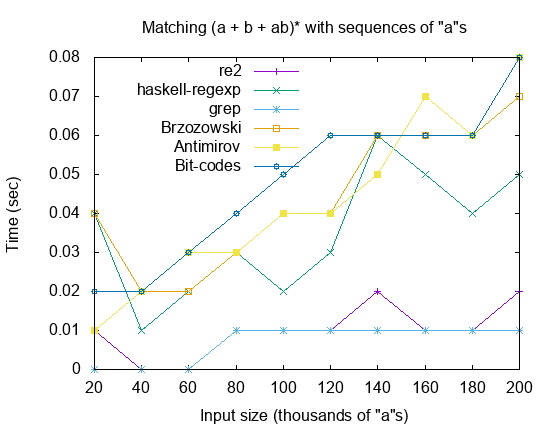
\includegraphics[width=0.9\textwidth]{as.png}
       \centering
       \caption{Results of experiment 1.}
       \label{fig:graph1}
     \end{figure}
   \end{frame}

   \begin{frame}{Future Work}
     \begin{itemize}
       \item How to improve efficiency?
       \begin{itemize}
         \item How intrinsic verification affects generated code efficiency?
         \item Currently porting code to use extrinsic verification (proofs separated from program code).
         \item Experiment with alternative formalization: BRE semantics defined by \ensuremath{\F{erase}}:
               \ensuremath{\V{s}\;\D{\in\langle}\;\V{e}\;\D{\rangle}\;\mathrel{=}\;\V{s}\;\D{\in\llbracket}\;\F{erase}\;\V{e}\;\D{\rrbracket}}.
       \end{itemize}
       \item How to measure memory consumption, without compiler support?
       \begin{itemize}
         \item No profiling support in Agda compiler.
         \item Agda compiles to Haskell, but there's no direct correspondence between
               Agda source code and Haskell generated code.
       \end{itemize}
     \end{itemize}
   \end{frame}

   \begin{frame}{Conclusion}
     \begin{itemize}
       \item We build a certified algorithm for BRE parsing in Agda.
       \item We certify several previous results about bit-coded parse trees and
             their relationship with RE semantics.
       \item Algorithm included in verigrep tool for RE text search.
     \end{itemize}
   \end{frame}

   \begin{frame}{Relating REs and BREs}
     \begin{itemize}
       \item Function \ensuremath{\F{fuse}} attach a bit-string into a BRE.
     \end{itemize}
     \begin{hscode}\SaveRestoreHook
\column{B}{@{}>{\hspre}l<{\hspost}@{}}%
\column{8}{@{}>{\hspre}l<{\hspost}@{}}%
\column{E}{@{}>{\hspre}l<{\hspost}@{}}%
\>[8]{}\F{fuse}\;\mathbin{:}\;\D{List}\;\D{Bit}\;\to \;\D{BitRegex}\;\to \;\D{BitRegex}{}\<[E]%
\\
\>[8]{}\F{fuse}\;\V{bs}\;\C{empty}\;\mathrel{=}\;\C{empty}{}\<[E]%
\\
\>[8]{}\F{fuse}\;\V{bs}\;(\C{eps}\;\V{x})\;\mathrel{=}\;\C{eps}\;(\V{bs}\;\F{++}\;\V{x}){}\<[E]%
\\
\>[8]{}\F{fuse}\;\V{bs}\;(\C{char}\;\V{x}\;\V{c})\;\mathrel{=}\;\C{char}\;(\V{bs}\;\F{++}\;\V{x})\;\V{c}{}\<[E]%
\\
\>[8]{}\F{fuse}\;\V{bs}\;(\C{choice}\;\V{x}\;\V{e}\;\V{e'})\;\mathrel{=}\;\C{choice}\;(\V{bs}\;\F{++}\;\V{x})\;\V{e}\;\V{e'}{}\<[E]%
\\
\>[8]{}\F{fuse}\;\V{bs}\;(\C{cat}\;\V{x}\;\V{e}\;\V{e'})\;\mathrel{=}\;\C{cat}\;(\V{bs}\;\F{++}\;\V{x})\;\V{e}\;\V{e'}{}\<[E]%
\\
\>[8]{}\F{fuse}\;\V{bs}\;(\C{star}\;\V{x}\;\V{e})\;\mathrel{=}\;\C{star}\;(\V{bs}\;\F{++}\;\V{x})\;\V{e}{}\<[E]%
\ColumnHook
\end{hscode}\resethooks
   \end{frame}

   \begin{frame}{Building bit-codes for $\epsilon$}
     \begin{hscode}\SaveRestoreHook
\column{B}{@{}>{\hspre}l<{\hspost}@{}}%
\column{8}{@{}>{\hspre}l<{\hspost}@{}}%
\column{E}{@{}>{\hspre}l<{\hspost}@{}}%
\>[8]{}\F{mkEps}\;\mathbin{:}\;\C{\lbrack\:\rbrack}\;\D{\in\llbracket}\;\V{t}\;\D{\rrbracket}\;\to \;\D{List}\;\D{Bit}{}\<[E]%
\\
\>[8]{}\F{mkEps}\;(\C{eps}\;\V{bs})\;\mathrel{=}\;\V{bs}{}\<[E]%
\\
\>[8]{}\F{mkEps}\;(\C{inl}\;\V{br}\;\V{bs}\;\V{pr})\;\mathrel{=}\;\V{bs}\;\F{++}\;\F{mkEps}\;\V{pr}{}\<[E]%
\\
\>[8]{}\F{mkEps}\;(\C{inr}\;\V{bl}\;\V{bs}\;\V{pr})\;\mathrel{=}\;\V{bs}\;\F{++}\;\F{mkEps}\;\V{pr}{}\<[E]%
\\
\>[8]{}\F{mkEps}\;(\C{cat}\;\V{bs}\;\V{pr}\;\V{pr'}\;\V{eq})\;\mathrel{=}\;\V{bs}\;\F{++}\;\F{mkEps}\;\V{pr}\;\F{++}\;\F{mkEps}\;\V{pr'}{}\<[E]%
\\
\>[8]{}\F{mkEps}\;(\C{star[]}\;\V{bs})\;\mathrel{=}\;\V{bs}\;\F{++}\;[\mskip1.5mu \;\C{1_b}\;\mskip1.5mu]{}\<[E]%
\\
\>[8]{}\F{mkEps}\;(\C{star-::}\;\V{bs}\;\V{pr}\;\V{pr'}\;\V{x})\;\mathrel{=}\;\V{bs}\;\F{++}\;[\mskip1.5mu \;\C{1_b}\;\mskip1.5mu]{}\<[E]%
\ColumnHook
\end{hscode}\resethooks
   \end{frame}
   \begin{frame}{Relating parse trees and RE semantics}
     \begin{itemize}
       \item \ensuremath{\F{unflat}} builds parse trees out of RE semantics evidence.
       \item Functions \ensuremath{\F{flat}} and \ensuremath{\F{unflat}} are inverses. 
     \end{itemize}
     \begin{hscode}\SaveRestoreHook
\column{B}{@{}>{\hspre}l<{\hspost}@{}}%
\column{8}{@{}>{\hspre}l<{\hspost}@{}}%
\column{E}{@{}>{\hspre}l<{\hspost}@{}}%
\>[8]{}\F{unflat}\;\mathbin{:}\;\V{xs}\;\D{\in\llbracket}\;\V{e}\;\D{\rrbracket}\;\to \;\D{Tree}\;\V{e}{}\<[E]%
\\
\>[8]{}\F{unflat}\;\C{\epsilon}\;\mathrel{=}\;\C{\epsilon}{}\<[E]%
\\
\>[8]{}\F{unflat}\;(\C{\$}\;\V{c})\;\mathrel{=}\;\C{\$}\;\V{c}{}\<[E]%
\\
\>[8]{}\F{unflat}\;(\V{prf}\;\C{\bullet}\;\V{prf'})\;\mathrel{=}\;\F{unflat}\;\V{prf}\;\C{\bullet}\;\F{unflat}\;\V{prf'}{}\<[E]%
\\
\>[8]{}\F{unflat}\;(\V{r}\;\C{+L}\;\V{prf})\;\mathrel{=}\;\C{inl}\;\V{r}\;(\F{unflat}\;\V{prf}){}\<[E]%
\\
\>[8]{}\F{unflat}\;(\V{l}\;\C{+R}\;\V{prf})\;\mathrel{=}\;\C{inr}\;\V{l}\;(\F{unflat}\;\V{prf}){}\<[E]%
\\
\>[8]{}\orange{\texttt{-- some code omitted}}{}\<[E]%
\ColumnHook
\end{hscode}\resethooks
   \end{frame}

\end{document}
 
